\documentclass[11pt,a4paper]{article}
\usepackage[T1]{fontenc}
\usepackage[utf8]{inputenc}
\usepackage{lmodern}
\usepackage[margin=2.3cm]{geometry}
\usepackage{graphicx}
\usepackage{booktabs}
\usepackage{longtable}
\usepackage{array}
\usepackage{xcolor}
\usepackage{enumitem}
\usepackage{caption}
\usepackage[colorlinks=true,linkcolor=blue!50!black,urlcolor=blue!50!black]{hyperref}
\setlist{itemsep=2pt,topsep=3pt}
\newcommand{\code}[1]{\texttt{\detokenize{#1}}}
\setlength{\parindent}{0pt}
\setlength{\parskip}{5pt}
\renewcommand{\arraystretch}{1.15}

\title{\textbf{PcbCreator}\\[2pt]\large Yerel Bir Dil Modeliyle Adım Adım PCB Şematik Tasarımı: Yöntem Raporu}
\author{PcbCreator projesi (TÜBİTAK 2209-A hazırlığı)\\\small Yazar listesi: TODO}
\date{20 Ekim 2026}

\begin{document}
\maketitle

\begin{abstract}
Bu rapor, PcbCreator sisteminin nasıl çalıştığını ve neden bu şekilde tasarlandığını anlatır. Sistem, yerelde çalışan nicemlenmiş bir 27B dil modeline (Ternary Bonsai 27B) küçük PCB şematiklerini \emph{blok blok} tasarlatır; her adımı deterministik bir linter, bir gözden geçirici model ve KiCad'in kendisi denetler. Literatürdeki yedi ilgili çalışmanın tam metni okunup yöntemimizle karşılaştırılmıştır. Gerçek çalıştırmalarda bulunan hata sınıfları ve her birine karşı eklenen önlemler tablo hâlinde verilmiştir. \textbf{Önemli not:} Gösterilen ilk başarılı tasarım henüz üretime hazır değildir (kondansatör değerleri datasheet'in altındadır); sonuçlar tek bir geliştirme isteği üzerindeki tek çalıştırmalardır ve bir kıyaslama değildir.
\end{abstract}

\section{Amaç ve kapsam}
Projenin hedefi, bir dil modelinin PCB'leri \emph{alt kartlar} hâlinde tasarlaması ve bu alt kartları tek bir kartta birleştirmesidir (uzun vadeli örnek: uçuş kontrol kartı). İlk aşamada hedef, birkaç basit kartın gerçekten üretilmesidir. Bu rapor yalnızca \textbf{şematik seviyesini} kapsar. Yerleşim, yönlendirme, tasarım kuralı kontrolü (DRC) ve üretim dosyaları (Gerber) henüz yapılmamıştır.

Tasarım ilkesi: \emph{tasarımı model yapar}. Parça seçimi, bağlantıların kurulması, değerlerin hesaplanması ve hataların düzeltilmesi modelin işidir. Koda ve insana düşen iş, modelin çıktısını \emph{denetlemek} ve resmî kaynakları (KiCad kütüphanesi, datasheet) ona sunmaktır. Elle yazdığımız örnek tasarımlar yalnızca test düzeneğidir ve modele hiçbir zaman gösterilmez.

\section{Genel bakış}
\begin{figure}[h]
\centering
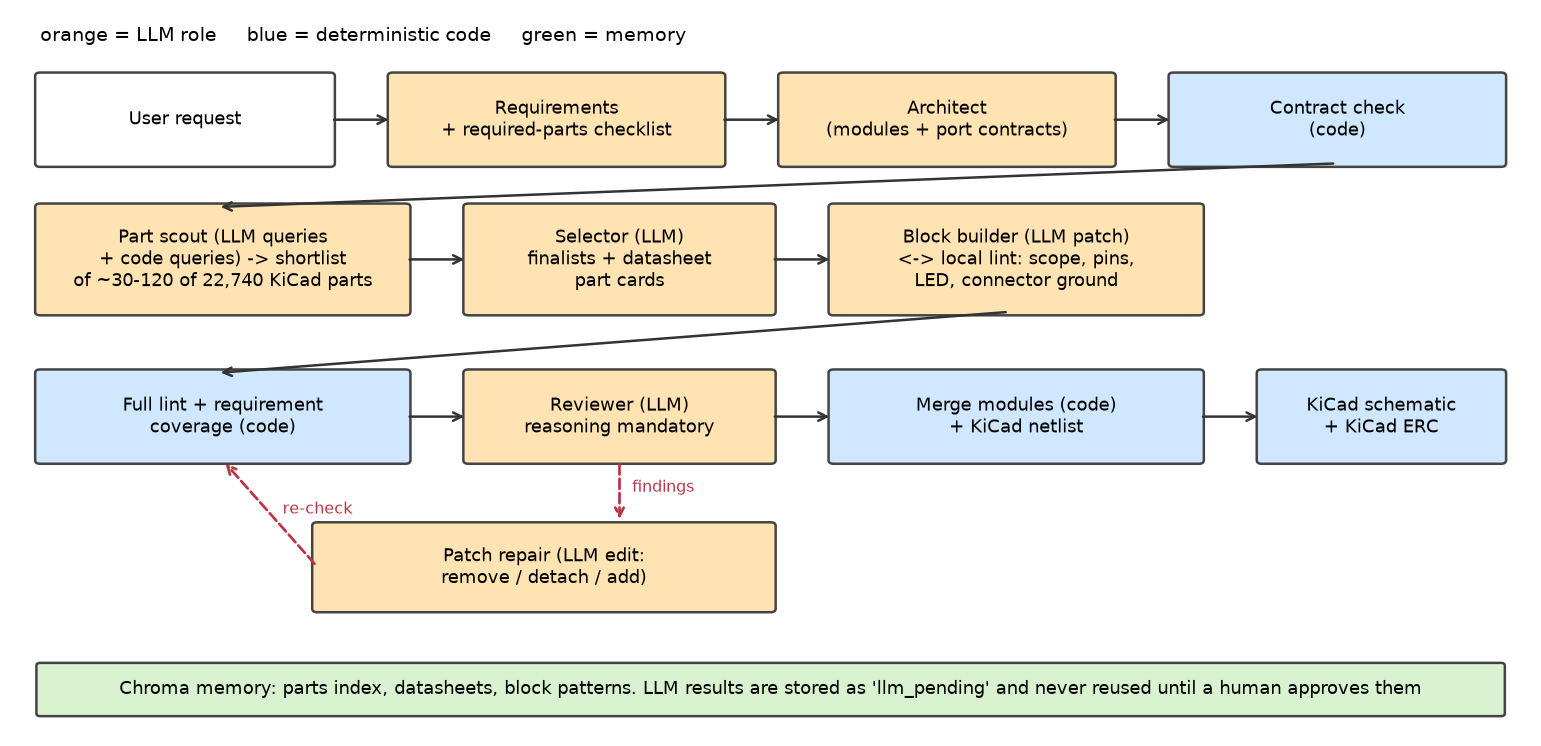
\includegraphics[width=0.97\textwidth]{../assets/architecture.png}
\caption{Sistem mimarisi. Turuncu: LLM rolleri, mavi: deterministik kod, yeşil: hafıza. Her LLM çıktısı ilerlemeden önce deterministik bir kapıdan geçer.}\label{fig:arch}
\end{figure}

Akış özetle şöyledir: kullanıcı isteği $\rightarrow$ gereksinim listesi $\rightarrow$ mimar (modüller ve port sözleşmeleri) $\rightarrow$ her modül için parça araması, finalist seçimi ve datasheet kartları $\rightarrow$ gereksinim listesinden \emph{koddan} türetilen bloklar $\rightarrow$ her blok için küçük bir yama ve hemen yerel denetim $\rightarrow$ tam denetim, gereksinim kapsaması ve gözden geçirici $\rightarrow$ gerekirse yama ile onarım $\rightarrow$ modüllerin birleştirilmesi $\rightarrow$ KiCad bağlantı listesi, şematik ve KiCad'in kendi denetimi.

\section{Yöntem}

\subsection{Veri modeli ve çalıştırılan kod yok}
Modelin ürettiği her şey doğrulanan JSON'dur (\code{Module}, \code{Net}, \code{Port}, \code{Design}); model çıktısı hiçbir zaman çalıştırılmaz. Bir modül; parçalar (referans, kütüphane kimliği, değer), netler (ad, pinler, gerilim, etiket) ve portlardan (modülün dış sözleşmesi) oluşur. Pinler \code{REF.PIN} biçiminde yazılır ve pin \emph{adıyla} verilmesi tercih edilir. Sunucu, JSON şemasına göre kısıtlı çözümleme yapar; böylece model yalnızca geçerli yapıda çıktı üretebilir, anlamsal geçerliliği ise linter denetler.

\subsection{Yerel model ve ortam}
Model: Ternary Bonsai 27B (PQ2\_0, yaklaşık 7,2~GB), PrismML'in llama.cpp çatalıyla (\code{llama-server}) sunulur; Ollama bu biçimi yükleyemez. Donanım: RTX 5060 (8~GB VRAM), 31~GB RAM. Katman dağılımı sunucunun otomatik sığdırmasına bırakılır (\code{-ngl 99} bellek yetmediği için çalışmadı). Ölçülen üretim hızı yaklaşık 6,5 token/sn, bağlam 16\,384 token. Her şey yerelde çalışır; dışarıya veri gönderilmez.

\subsection{Gereksinimler ve kontrol listesi}
İlk rol, isteği bir gereksinim kaydına çevirir ve \emph{gerekli parçalar kontrol listesi} çıkarır (\code{connector}, \code{linear_regulator}, \code{switching_regulator}, \code{led}, \code{mcu}, \code{sensor}, \code{support}, \code{other}; adet ve açıklama ile). \code{support} türü, yalnızca başka bir parçaya hizmet eden direnç ve kondansatörler içindir (örneğin LED'in direnci) ve kendi bloğunu almaz. Bu tür, gerçek bir çalıştırmada direncin ayrı bir madde olarak yazılıp LED bloğunun iki kez kurulmasından sonra eklenmiştir. Kontrol listesi hem blokları türetir hem de sonda kapsama denetiminin ölçütüdür (PCBSchemaGen'in "gerekli bileşen kümesi" fikriyle uyumlu).

\subsection{Mimar ve port sözleşmeleri}
Mimar, kartı modüllere böler ve her modülün portlarını yazar: ad, yön (\code{in/out/bidir/power_in/power_out}), tür (\code{signal/power/ground}), gerilim. Sözleşmenin kendisi modül tasarlanmadan önce doğrulanır (güç portu \code{power_in/power_out} yönünde ve gerilimli olmalı, toprak \code{bidir} olmalı). Bu kontrol, mimarın geçersiz sözleşme yazıp modül tasarımcısını çözülemez bir çelişkiye soktuğu bir koşunun ardından eklenmiştir. Tek modüllü kartlarda \code{links} ve \code{expose} alanları portlardan koda türetilir, çünkü bağlanacak başka modül yoktur; bu, modelin çıktısının üzerine yazılan tek yerdir.

\subsection{Parça seçimi: 22.740 parçadan kısa listeye}
Parça kaynağı, KiCad 10'un resmî sembol kütüphanesidir. Bir içe aktarıcı, \code{.kicad_sym} dosyalarını okur: pin numaraları, adları ve elektriksel türler doğrudan resmî kütüphaneden gelir, modelin uydurması gerekmez. KiCad'in toprak pinlerini \code{power_in} diye işaretlediği düzeltilir; genel pasiflere 0805 gibi elle lehimlenebilir varsayılan footprint atanır. Toplam 22.740 parça yaklaşık 15~sn'de okunur.

Tüm parçalar Chroma'ya anlamsal gömme (all-MiniLM-L6-v2, yerel) ile indekslenir. Model 22.740 parça arasından doğrudan seçim yapmaz: önce arama sorguları üretilir (modelin sorguları \emph{ve} gereksinim listesinden koddan türetilen sorgular; modelin sorgularının kırılgan olduğu görülmüştür), her sorgu ilk 30 adayı getirir, sonuçlar harmanlanarak yaklaşık 30--120 parçalık bir \emph{kısa liste} oluşur. Sonra bir seçici model çağrısı, gerekçesini yazarak en fazla sekiz finalist seçer; listede olmayan kimlikler kodla atılır. Direnç, kondansatör, LED ve pin başlığı konnektörleri her zaman sunulur ve aranmaz (arama bunlar için gürültü getirmiştir: XLR jakları, şebeke fişleri, RGB LED'ler).

\subsection{Datasheet parça kartları}
Finalist entegreler için datasheet PDF'i indirilir (üreticiler betik istemcilerini engelleyebilir; bu durumda PDF elle \code{datasheets_manual} klasörüne konur), \code{pdftotext} ile ilk 40 sayfa metne çevrilir, parçalanır ve Chroma'ya yazılır. Birden fazla hedefli arama (pinler, gerilim aralığı, giriş kondansatörü, çıkış kondansatörü, tipik uygulama) birleştirilerek modele sunulur ve model yapılandırılmış bir \emph{parça kartı} çıkarır: tür, giriş/çıkış gerilimi, dropout, azami akım, \textbf{asgari giriş ve çıkış kapasitansı}, gerekli dış parçalar, pin notları. Literatürdeki çalışmaların hiçbiri datasheet'i ham metin olarak vermez; hepsi yapılandırır (pcbGPT, HWE-Bench, PCBSchemaGen, DRCY).

Kart değerlerini \emph{model} çıkarır; bu nedenle onaylanmamış sayılır. Bir çalıştırmada modelin kartında kendi kendine \code{confirmed: true} yazdığı görüldü; artık kod bu alanı her zaman \code{false} yapar ve yalnızca bir insan, datasheet'i kontrol ettikten sonra elle değiştirebilir. Kartlarda sayısal hatalar da görüldü (bir regülatör için 800~mA yerine ``800~A'' yazıldı).

\subsection{Adım adım blok kurma}
Tek seferde bütün modülü yazdırmak yerine, kontrol listesinden \emph{koddan} türetilen her blok için (regülatör, LED, her konnektör) model küçük bir \emph{yama} üretir: yeni parçalar ve bu bloğun nete eklediği pinler. Adımlar koddan gelir çünkü modelin kendi bölmesini icat etmesi güvenilir değildir (ROME çalışması da aynı bulguyu bildirir). Port netleri, mimarın sözleşmesinden koda kopyalanır; model bunları her adımda yeniden yazmak zorunda değildir.

Her yama uygulanınca \emph{yerel lint} çalışır: yalnızca yeni parçalar ve dokunulan netler hakkında, ve yalnızca kısmi bir modülde hükmedilebilen kural aileleri (bilinmeyen parça ve pin, çift referans, bağlantısız pin, çıkış çakışması, LED, konnektör toprağı, datasheet kapasitans asgarisi). Bulgular pin düzeyindedir ve modele geri verilir. Ek olarak \textbf{kapsam kuralı} vardır: bir blok yalnızca kendi türünden parça ekleyebilir (regülatör bloğuna LED eklenemez). Bir blok altı denemede temizlenemezse zincir sürdürülmez, durum modül düzeyindeki onarım döngüsüne devredilir.

\subsection{Tam denetim, kapsama ve gözden geçirici}
Tüm bloklar bitince modül tam linter'dan, port sözleşmesi kontrolünden ve gereksinim kapsama denetiminden geçer. Kapsama, parçaları KiCad kütüphane ailesine göre sayar (örneğin \code{Regulator_Linear} ile \code{Regulator_Switching} ayrıdır); böylece ``lineer LDO'' isteğine anahtarlamalı regülatör konması yakalanır. Linter'dan geçen modül, \emph{gözden geçirici} role gider: gereksinimleri, datasheet kartlarını ve devrenin metin dökümünü görür; muhakemesini yazmak zorundadır (LED için akım yolunu rayından toprağa yazar) ve gerçek sorunları listeler. Gözden geçirici deterministik değildir ve linter'dan ayrı tutulur.

\subsection{Yama tabanlı onarım}
Denetimden bulgu gelirse model modülü baştan yazmaz; yalnızca \emph{silinecek parçalar}, \emph{ayrılacak pinler} ve \emph{eklenecek parça/bağlantılar} içeren en küçük düzenlemeyi üretir (pin eşlemesi çözülmüş numaralarla yapılır: \code{U1.EN} ile \code{U1.3} aynıdır). Bu yöntem, tam yeniden yazımın çalışan parçaları bozduğu bir çalıştırmadan sonra benimsenmiştir (SchGen de çıktıyı düzenleme komutları dizisi olarak ele alır).

\subsection{Modüllerin birleştirilmesi}
Birleştirme deterministik koddur. Bağlantılar \code{modül.net} biçiminde yazılır; port türü, yönü, gerilimi ve protokolü birbirini tutmalı, her ağda tek sürücü olmalı, her gerekli port bağlanmalı veya dışarıya açıkça verilmelidir (kurallar E100--E107, sözleşme denetimi E110--E112). Tüm \code{GND} netleri tek toprak olur, referanslar yeniden numaralandırılır. Birleşik kart yeniden denetlenir; bu, tek bir modülün göremeyeceği hataları (örneğin I2C hattında hiçbir modülde bulunmayan pull-up) yakalar.

\subsection{KiCad çıktıları ve bağımsız doğrulama}
Sistem KiCad bağlantı listesi (\code{.net}) ve gerçek bir KiCad şematiği (\code{.kicad\_sch}) üretir. Şematikte parçalar sinyal akışı boyunca sütunlara dizilir, her net için sütunlar arasına dikey bir bara çekilir ve her pin ona bağlanır; birden fazla sütuna yayılan netler üstte bir köprü kablosuyla birleştirilir (toprak tek merkezi hat olur). Çizim, KiCad'in \code{kicad-cli} ile bağlantı listesini yeniden dışa aktarması ve bizimkiyle karşılaştırılmasıyla \emph{doğrulanır}; uyuşmazlıkta başka yerleşim varyantları denenir, hiçbiri uymazsa her zaman doğru olan etiket stiline dönülür. Çizimden KiCad'in kendi ERC'si, PDF ve PNG de alınır. Bu çizim, linter'ın ve gözden geçiricinin geçirdiği iki hatalı tasarımı ortaya çıkarmıştır (Bölüm~\ref{sec:bulgu}).

\subsection{Hafıza ve insan onayı}
Chroma'da parçalar, datasheet parçaları ve blok kalıpları saklanır. Her kaydın kaynağı vardır: \code{human} (elle yazılmış genel kalıplar), \code{llm\_pending} (model sonucu, henüz onaylanmamış), \code{llm} (insan onayı sonrası). \code{llm\_pending} kayıtlar aramalardan hariç tutulur; \code{pcbc pending} ve \code{pcbc approve} ile insan onayı gerekir. Bu kural, yanlış iki tasarımın ``doğrulanmış'' diye hafızaya yazılmasından sonra konmuştur. Hafızadaki örnekler tüm kartlar değil \emph{blok kalıplarıdır} (LED + seri direnç, IC + dekuplaj kondansatörü, I2C pull-up, regülatör aşaması).

\section{Linter kuralları}
\begin{longtable}{@{}p{1.7cm}p{14cm}@{}}
\toprule \textbf{Kural} & \textbf{Ne denetler} \\ \midrule \endhead
E001--E005 & Bilinmeyen parça (``\code{Device:R} mi demek istedin?'' önerisi ile), bilinmeyen/belirsiz pin, bir pinin iki nette olması, çift referans, çift net adı \\
E010 & Bağlantısız pin (NC pin hariç) \\
E020--E023 & Güç girişi olan netin kaynağı yok, beslenen pinin gerilim aralığı dışı, aynı netde birden çok güç çıkışı, bildirilen gerilim uyumsuz \\
E030--E032 & Aynı netde birden çok çıkış, çıkış ile gelen port çatışması, sürücüsüz giriş \\
E040 & IC güç pininin toprağa dekuplaj kondansatörü yok \\
E050 & I2C hattında pull-up yok (birleşik kartta uygulanır) \\
E051 & LED iki ray arasında doğrudan, ya da seri direnç yok (direnç paralel de olsa yakalanır) \\
E053 & Hat taşıyan konnektörde toprak pini yok \\
E054 & Giriş/çıkış kapasitansı, datasheet kartındaki asgarinin altında \\
E060--E061 & Toprak pini toprak olmayan netde \\
E070--E073 & Port ve net uyumu, güç portu gerilimi, port yön/tür kuralları \\
E200 & Gereksinim listesindeki parça yok veya türü yanlış \\
E205 & Blok kapsamı: bir bloğa başka bloğun parçası eklenmiş \\
E090 & (\code{--strict}) Doğrulanmamış parça \\ \bottomrule
\end{longtable}

\section{Literatürle karşılaştırma}
Tam metni okunan çalışmalar ve yöntemimizle ilişkileri aşağıdadır. Sayılar makalelerin kendi bildirimidir; başvuruda kullanmadan önce kaynaktan yeniden doğrulanmalıdır.

\begin{longtable}{@{}p{3.1cm}p{6.6cm}p{6.2cm}@{}}
\toprule \textbf{Çalışma} & \textbf{Ne yapıyor / bulgu} & \textbf{Bizdeki karşılığı} \\ \midrule \endhead
pcbGPT [1] & Python DSL ile KiCad şematiği; ajan arama aracını kendisi çağırır; datasheet'ten \emph{tasarım özeti}; ERC sonrası ayrı bir \emph{doğrulama ajanı}; 20 görevde pass@1 0,90, zor görevlerde 0,72 & Parça kartları, ayrı gözden geçirici. Fark: biz arama sonucunu istemde veriyoruz, ajan aracı değil \\
PCBSchemaGen [2] & Eğitimsiz; 5 katmanlı deterministik doğrulayıcı, pin düzeyinde hata yerelleştirme, aday popülasyonu ve bandit; açık 31B model PCBBench'te \%81,3; kompakt bağlam (18k token) \%78,0, tam kütüphane (35k) \%73,7; doğrulayıcı ve istemler değerlendirmeden önce donduruluyor & Linter, pin düzeyinde geri bildirim. Eksik: aday popülasyonu, donmuş test seti \\
CircuitLM [3] & Gömme tabanlı bileşen bilgi tabanı; deterministik ERC ve LLM-hakem; ERC'de \%88 geçen model hakemde \%53; parça yoksa insana dur; CoT planlama & ERC ile hakemin ayrı olması, parça yoksa durma \\
HWE-Bench [4] & 300 kart ölçeğinde görev; en iyi model \%8,15; datasheet JSON'a çevrilir; sinyal zinciri ve protokol sözleşmeleri hataları azaltır & Port sözleşmeleri, yapılandırılmış kart \\
SchGen [5] & Düzenleme komutları dizisi olarak çıktı; pin adıyla bağlantı kritik; CoT çıkarılınca geçerli devre \%82,0'dan \%53,4'e & Pin adı tercihi, yama tabanlı onarım, muhakeme alanı \\
DRCY [6] & Datasheet çıkarımı puanlanır, 5 deneme, önbellek; çok koşulu uzlaşı & Kart önbelleği; uzlaşı yok \\
DEVICES [7] & LLM sayısal hesap yapmaz, betik üretir; modüler aşamalar bağlamı 8,6 kat azaltır & Adım adım bağlam azaltma; hesabı kod doğrular (kısmen) \\
ROME [8], Yin vd. [9] & Aşamalı istem düz isteme göre zayıf modellere en çok yarar; modelin kendi bölmesini icat etmesi güvenilmez; kompakt JSON durum özeti & Bloklar koddan türetilir; durum özeti \\ \bottomrule
\end{longtable}

\textbf{Yeni olduğunu düşündüğümüz noktalar} (aranan çalışmalarda bulunamadı; kapsamlı bir tarama değildir): (i) PCB'yi alt kartlara bölüp port sözleşmeleriyle birleştirme, (ii) uçuş kontrol kartı gibi İHA donanımı, (iii) kart çizimini KiCad'in kendi bağlantı listesiyle her seferinde doğrulama.

\section{Gerçek çalıştırmalardan bulgular}\label{sec:bulgu}
Tüm çalıştırmalar tek bir geliştirme isteği üzerindedir: 5~V girişten 3,3~V üreten düşük dropout lineer regülatör, giriş ve çıkış için iki 2 pinli konnektör, ve çıkışta yaklaşık 2~mA'lik yeşil bir LED. Model deterministik değildir (sıcaklık 0,3).

\begin{longtable}{@{}p{7.4cm}p{8.6cm}@{}}
\toprule \textbf{Yerel modelin hatası} & \textbf{Önlem} \\ \midrule \endhead
Lineer istenen yerde anahtarlamalı regülatör seçti & Kütüphane ailesine göre kapsama denetimi (E200) \\
Arama sorgularını ``led'', ``resistor'' gibi boş etiketlerle yazdı & Sorgular gereksinim listesinden koddan da üretilir \\
LED'i doğrudan 3,3~V ile toprak arasına, direnci paralel bağladı; linter ve gözden geçirici geçirdi & E051 kuralı; gözden geçiriciye zorunlu muhakeme \\
İki 2 pinli konnektörü VIN/VOUT bağladı, toprak yok; yine geçti & E053 kuralı; \textbf{çizim} hatayı gösterdi \\
Gereksinim listesinde LED direncini ayrı madde yazdı, LED bloğu iki kez kuruldu & \code{support} türü \\
Regülatör bloğuna LED ekledi; sonraki bloklar çakıştı & Blok kapsam kuralı (E205); kirli blok onarıma devredilir \\
Tüm modülün yeniden yazımı çalışan parçaları bozdu & Yama tabanlı onarım \\
Mimar geçersiz port sözleşmesi yazdı (güç portu \code{in/out}) & Sözleşme doğrulaması, port şemasına açıklamalar \\
Yanlış tasarımlar iki kez ``doğrulanmış'' diye hafızaya yazıldı & \code{llm\_pending} ve insan onayı \\
Kendi kartında \code{confirmed: true} yazdı & Kod bu alanı her zaman \code{false} yapar \\
Mimar istemindeki örnek modül adlarını (``mcu'', ``sensors'') kopyaladı & İstemden örnekler kaldırıldı (bu bizim hatamızdı) \\ \bottomrule
\end{longtable}

\subsection{Sonuç 1: tüm kapılardan geçen ilk tasarım}
Dört blok (regülatör, LED, iki konnektör) ilk denemede kabul edildi; modül tam linter'dan, kapsama denetiminden ve gözden geçiriciden geçti; KiCad dosyayı açıp çiziyor ve bağlantı listesi bizimkiyle birebir uyuyor (Şekil~\ref{fig:s1}). Model, LED direncini (3,3--2,0)/2~mA $\approx$ 650~$\Omega$ diye hesaplayıp standart 620~$\Omega$ seçti (akım yaklaşık 2,1~mA).

\textbf{Ama tasarım hâlâ yanlıştır.} Parçanın datasheet'ini (TI LP38693) elle okuduk: giriş kondansatörü için 1~$\mu$F ``kararlılık için gerekli'', çıkış için en az 1~$\mu$F seramik isteniyor. Modelin koyduğu iki kondansatör 100~nF'tır; regülatör kararsız çalışabilir. Bunun nedeni, datasheet'in yalnızca ilk 12 sayfasını okuyup uygulama bölümünü (daha sonraki sayfalar) kaçırmamızdı. Okuma 40 sayfaya çıkarıldı, kartlara asgari kapasitans alanları ve E054 kuralı eklendi; ancak yeni kartlar henüz bu hatayı tutarlı biçimde yakalayacak kadar güvenilir değildir.

\begin{figure}[h]
\centering
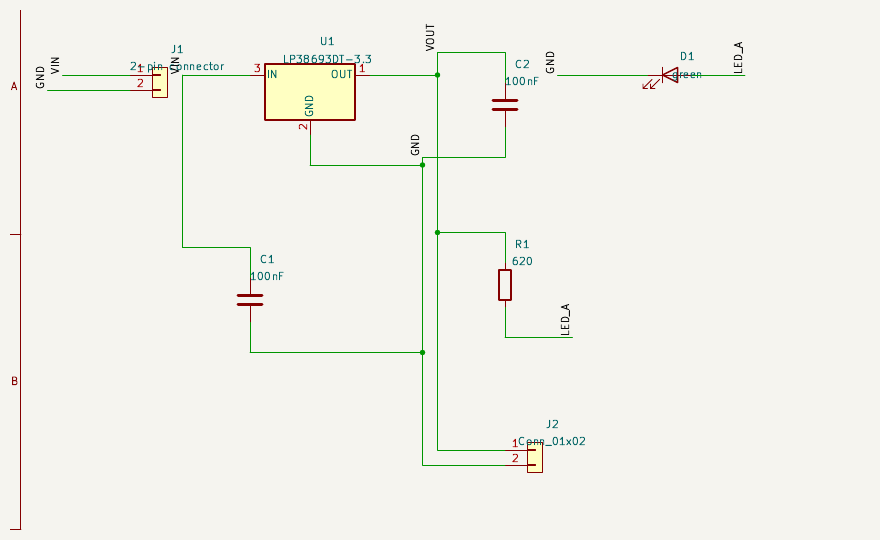
\includegraphics[width=0.82\textwidth]{../plots/sonuc_1.png}
\caption{Yerel modelin tasarladığı, KiCad'in çizdiği 5~V$\rightarrow$3,3~V LDO kartı. Üretime hazır değil: C1 ve C2 değerleri datasheet asgarisinin altında.}\label{fig:s1}
\end{figure}

\subsection{Sonuç 2: linter ve gözden geçiriciden geçen yanlış tasarım}
Daha önceki bir tasarım hem linter'dan hem gözden geçiriciden geçti, oysa iki konnektör de VIN/VOUT'a bağlıydı ve hiçbirinde toprak yoktu. Hata, tasarım \emph{çizilince} bir bakışta anlaşıldı (Şekil~\ref{fig:s2}). Bu, CircuitLM'in bulgusuyla uyumludur (kural tabanlı denetim geçse de anlamsal denetim çok daha fazla kusur bulur) ve her hata sınıfı için deterministik kural eklememizin gerekçesidir.

\begin{figure}[h]
\centering
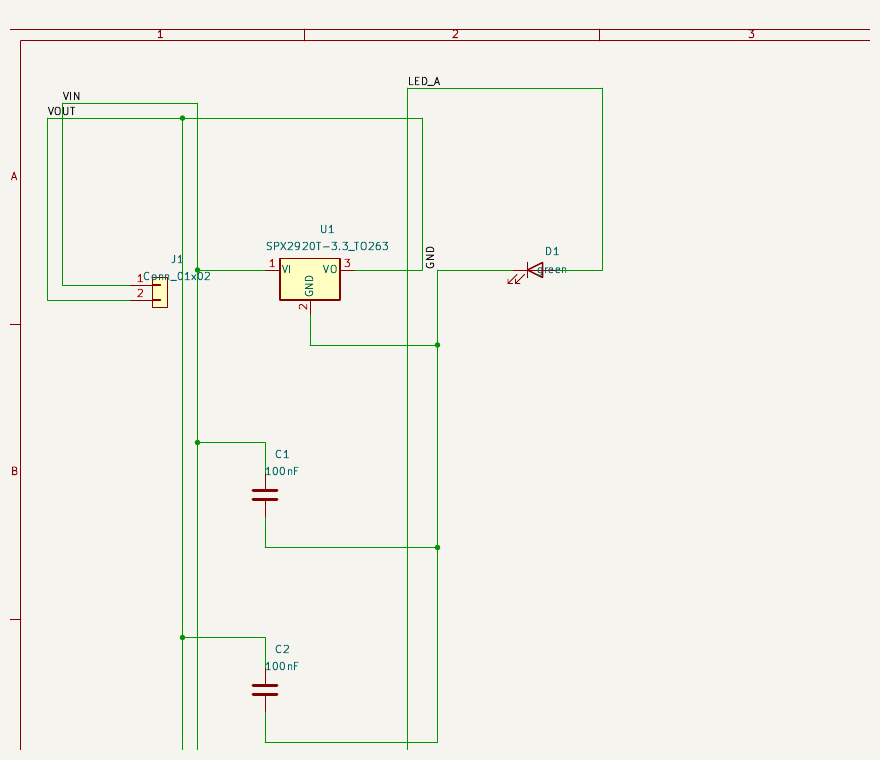
\includegraphics[width=0.62\textwidth]{../plots/sonuc_2.png}
\caption{Linter ve gözden geçiriciden geçen ama yanlış tasarım: konnektörlerde GND yok.}\label{fig:s2}
\end{figure}

\section{Sınırlamalar ve dürüstlük notu}
\begin{itemize}
\item Tüm bulgular tek isteğin, tek modelin tek çalıştırmalarıdır. İstemler ve kurallar aynı geliştirme isteğinde görülen hatalara göre ayarlandı; \textbf{genelleme kanıtı yoktur}. Dondurulmuş, görülmemiş bir test seti ve $k$ koşulu başarı oranları gerekir (PCBSchemaGen'in yöntemi).
\item Literatürdeki çalışmaların görevleri gerekli entegreleri veriyor; bizim model 22.740 parça arasından kendi seçiyor, bu daha zor bir ayardır. Sayılar doğrudan karşılaştırılamaz.
\item Datasheet kartları zayıf ve model çıkarımıdır; sayısal ve birim hataları görüldü. Elektriksel sınırlar, bir insan datasheet'i kontrol edene kadar doğrulanmış değildir. Üretime giden kartta \code{--strict} ve uzman incelemesi zorunludur.
\item Bazı üreticiler (örneğin analog.com, liteon) betik indirmelerini engelliyor; PDF elle konmalıdır.
\item Yalnızca şematik: yerleşim, yönlendirme, DRC ve Gerber yoktur. Seed parça kütüphanesi basitleştirilmiş ve doğrulanmamıştır; elle yazılmış uçuş kartı yalnızca linter/birleştirici testidir.
\item Şematik çiziminde okunabilirlik iyileştirilebilir (uzun dikey sütunlar, köprü kabloları); bağlantıların doğruluğu KiCad ile doğrulanır, güzelliği değil.
\end{itemize}

\section{Sonraki adımlar}
\begin{enumerate}
\item Çok modüllü kartlar (güç + sensör + MCU, sonra uçuş kontrol kartı) ile birleştirme hattının gerçek modelle denenmesi.
\item Dondurulmuş test seti ve pass@$k$ ile başarı oranları; aday popülasyonu, sürekli skor ve uyarlanabilir sıcaklık (PCBSchemaGen), çok koşulu uzlaşı (DRCY).
\item Datasheet kartlarının iyileştirilmesi ve insan onaylı kart akışı.
\item Yerleşim (modelin kısıt vermesi, algoritmanın yerleştirmesi), Freerouting ile yönlendirme, \code{kicad-cli} ile DRC ve Gerber; insan onayıyla ilk basit kartın üretimi.
\item Elle seçilmiş blok kalıplarının KiCad şablonlarından ve açık donanım projelerinden otomatik genişletilmesi (kalite kapısı ve lisans izi ile).
\end{enumerate}

\section{Yeniden üretme}
Kod ve bu rapor: \url{https://github.com/GulogluHaktan/PcbCreator}. Testler: \code{uv run pytest} (model gerekmez). Gösterilen çizimler: \code{uv run pcbc render results/ldo_board.module.json}. Model sunumu: \code{scripts/serve.sh}. Tam çalıştırma: \code{uv run pcbc design "..." --kicad}. Ayrıntılı adımlar depodaki README dosyalarındadır.

\section*{Kaynaklar}
\begin{small}
\begin{enumerate}[label={[\arabic*]},leftmargin=1.2cm]
\item King, Kehrberg, Beigl, R\"oddiger. pcbGPT: Automatic PCB Schematic Synthesis from Natural Language Requirements. arXiv:2606.01188, 2026.
\item Zou vd. PCBSchemaGen: Reward-Guided LLM Code Synthesis for PCB Schematic Design with Structured Verification. arXiv:2602.00510, 2026.
\item Al Hasan vd. CircuitLM: A Multi-Agent LLM-Aided Design Framework for Generating Circuit Schematics from Natural Language Prompts. arXiv:2601.04505, 2026.
\item Qiu, Xiao, Pan. HWE-Bench: Can Language Models Perform Board-level Schematic Designs? arXiv:2603.18102, 2026.
\item Luo, Ma, Zhang, Qiu. SchGen: PCB Schematic Generation with Semantic-Grounded Code Representations. arXiv:2605.30345, 2026.
\item Dumont vd. DRCY: Agentic Hardware Design Reviews. arXiv:2603.15672, 2026.
\item Qiao, Dick. LLM-Driven, Datasheet-Aware Automated Hardware Compatibility Verification for Early-Stage, Pre-Schematic Embedded System Design. arXiv:2608.25217, 2026.
\item Nakkab, Zhang, Karri, Garg. Rome was Not Built in a Single Step: Hierarchical Prompting for LLM-based Chip Design. arXiv:2407.18276, 2024.
\item Yin vd. LLM-based Hardware Development with Hierarchical IRs and End-to-End Multi-Agent Workflow. arXiv:2608.30659, 2026.
\item Srinivasan, Turnbull, Pearce. Surveying GenAI-based Automation in Printed Circuit Board Design and Test. arXiv:2606.17074, 2026.
\end{enumerate}
\end{small}

\end{document}
